\section{Projektinitialisierung}
\subsection{Ausgangslage}

Die Firma ImmoGlobal verwaltet im Auftrag ihrer Kunden Wohnliegenschaften in der ganzen Schweiz. Sie beschäftigt insgesamt 30 Personen in der Administration, 20 davon am Hauptsitz in Bern und je 5 in Lausanne und Zürich. Hinzu kommen Hauswartungspersonen, die für eine oder mehrere Liegenschaften zuständig sind. Die Aktivitäten im Tessin werden von Zürich aus gesteuert.
Das Aufgabenspektrum von ImmoGlobal umfasst folgende Aktivitäten:
\begin{itemize}
  \item Vermietung der verschiedenen Mietobjekte (Wohnungen, Räume, Garagen und Parkplätze)
  \item Erstellung und Verwaltung der Mietverträge.
  \item Übergabe der Mietobjekte an die neuen Mieter (inkl. Übergabeprotokoll)
  \item Mietzinsinkasso (inkl. Kontrolle und Mahnung)
  \item Abrechnung der Nebenkosten
  \item Führen einer einfachen Buchhaltung der Ein- und Ausgaben
  \item Instandhaltung der Gebäude (Reparaturen und Renovationsarbeiten werden extern in Auftrag gegeben)
  \item Rücknahme der Mietobjekte nach Ablauf des Mietverhältnisses (inkl. Übernahmeprotokoll)
\end{itemize}

\subsection{Situationsanalyse (IST-Zustand)}
ImmoGlobal arbeitet heute mit einer veralteten, eigenentwickelten Software sowie mit den gängigen Microsoft Office-Produkten (Word, Excel und Outlook). Diese Lösung ist nicht mehr zeitgerecht und muss angesichts des Wachstums der Firma in naher Zukunft ersetzt werden. Der Geschäftsführer von ImmoGlobal hat verschiedene, auf dem Markt verfügbare, Standardsoftware für die Verwaltung von Liegenschaften an-geschaut, erachtet sie aber als zu kompliziert. Er bevorzugt eine einfache, auf die Bedürfnisse von ImmoGlobal zugeschnittene Lösung und beauftragt Sie deshalb eine solche Software zu entwickeln.\\
Die Software soll den Geschäftsführer:innen und seinen Mitarbeiter:innen einen besseren Überblick über die zu verwaltenden Liegenschaften und Objekte erlauben, die Effizienz steigern sowie die zuhanden der Kunden zu liefernden Abrechnungen automatisieren.\\
Basierend auf den Angaben im vorliegenden Dokument ist zuerst ein Pflichtenheft zu erstellen. Dabei sind die vorliegenden Informationen auf ihre Vollständigkeit hin zu überprüfen. Allfällige Lücken müssen im Hinblick auf das Verfassen des Pflichtenhefts geschlossen werden. Anschliessend ist auf der Basis des von Ihnen erstellten Pflichtenhefts ein Prototyp der Applikation zu entwickeln.

\subsection{Anforderungen}
Jede Liegenschaft wird durch eine eindeutige Nummer gekennzeichnet und beinhaltet verschiedene Objekte (Wohnungen, Räume, Garagen oder Parkplätze), welche wiederum eine eindeutige Kennzeichnung innerhalb der Liegenschaft aufweisen.\\
Für jedes Objekt können mehrere Mietverträge im System vorhanden sein, wobei zu einem bestimmten Zeitpunkt nur einer gültig sein darf. Für jeden Mietvertrag werden die geschuldeten und effektiv bezahlten Mietzinse und Nebenkostenanteile auf entsprechenden Konten gebucht, so dass eine Übersicht über die ausstehenden Beträge jederzeit erstellt werden kann.\\
Bei den Kreditorenrechnungen wird zwischen solchen, die ein bestimmtes Objekt betreffen, und solchen, welche die Liegenschaft als Ganzes betreffen, unterschieden. Dementsprechend muss jede Rechnung entweder einem Objekt oder einer Liegenschaft zugeordnet und auf ein entsprechendes Konto gebucht werden.\\

\newpage
Der Prototyp muss mindestens folgende Funktionalität (MUSS-Kriterien) abdecken:
\begin{itemize} \label{musskrit}
  \item Mandantenfähigkeit
  \item Verwaltung von Liegenschaften
  \item Verwaltung von Objekten
  \item Verwaltung von Mieter/innen
  \item Verwaltung von Mietverträgen (nur Inhalt, siehe unten)
  \item Mietzinsinkasso / Verbuchung der Mietzinse auf den entsprechenden Konten
  \item Mietzinskontrolle (inkl. Mahnung)
  \item Erfassen der Kreditorenrechnungen / Verbuchung auf unterschiedliche Konten
\end{itemize}

\vspace{3mm}
Gewünschte, zusätzliche Funktionalität (SOLL-Kriterien):
\begin{itemize}
  \item Mehrsprachigkeit
  \item Übergabeprotokoll bei der Übergabe des Mietobjekts
  \item Übernahmeprotokoll bei der Rücknahme des Mietobjekts
  \item Nebenkostenabrechnung (Zusammenzug der entsprechend gekennzeichneten Rechnungen pro Konto für eine bestimmte Periode)
  \item Nebenkosteninkasso / Verbuchung auf den entsprechenden Konten
  \item Kontrolle des Nebenkosteninkassos (inkl. Mahnung)
\end{itemize}

\vspace{3mm}
Der Prototyp muss mindestens folgende Informationen verwalten können:
\begin{itemize}
  \item Liegenschaft
  \begin{itemize}
    \item Identifikation (nummerisch, frei wählbar)
    \item Bezeichnung
    \item Liegenschaftsadresse
    \item Anzahl Objekte je Kategorie (Wohnung, Raum, Garage oder Parkplatz)
    \item Für die Liegenschaft abgeschlossene Versicherungen (insb. Gebäude-, Haftpflicht- und Personenversicherungen).
    \item Hauswartungsperson
  \end{itemize}
  \newpage
  \item Objekt
  \begin{itemize}
    \item Identifikation (frei wählbar)
    \item Bezeichnung
    \item Lage (frei wählbar, z.B. «1. OG links», «1. OG Mitte», «1. OG rechts»)
    \item Anzahl Zimmer (für Wohnungen)
    \item Fläche (in m2)
    \item Objektbeschreibung (freier Text)
    \item Kühlschrank \footnotemark{}
    \item Geschirrwaschmaschine\footnotemark[\value{footnote}]
    \item Kochherd/Backofen \footnotemark[\value{footnote}]
    \item Waschmaschine\footnotemark[\value{footnote}]
    \item Tumbler\footnotemark[\value{footnote}]
    \item Anzahl Schlüssel je Kategorie (Haus-, Wohnungs-, Briefkasten-, Waschküche-, Keller-, Estrichschlüssel, usw.)
    \footnotetext{Mindestanforderung: Ja/Nein; Erweiterung: Marke, Modell, Lieferdatum}
  \end{itemize}

  \item Mieter:in
  \begin{itemize}
    \item Name, Vorname 
    \item Geburtsdatum
    \item Heimatort 
    \item Zivilstand
    \item Vorherige Adresse
    \item Telefonnummer (privat, mobil, beruflich)
    \item Email-Adresse (privat, beruflich)
    \item Bank-/Postverbindung
  \end{itemize}
  \item Mietvertrag
  \begin{itemize}
    \item Mieter:in
    \item Liegenschaft / Objekt
    \item Mietbeginn und gegebenenfalls Mietende
    \item Monatlicher Mietzins, monatliche Nebenkosten
    \item Art der Nebenkosten (Pauschal bzw. Akonto)
    \item Auflistung der Kostenarten, welche über die Nebenkosten abgerechnet werden (Heiz-, Warmwasseraufbereitungs-, Wasser-, Hauswart-, Treppen-reinigungs-, Gartenarbeits-, Strom-, Lift-, Kabelfernsehkosten sowie Abwasser- Kehrichtgebühren)
    \item Mietdepot (Ja/Nein) und Depotbetrag in CHF
  \end{itemize}
 
  \item Rechnungen
  \begin{itemize}
    \item Konto (nummerisch, mindestens vierstellig)
    \item Kreditor
    \item Rechnungsdatum
    \item Fälligkeitsdatum
    \item Zweck
    \item Liegenschaft / Objekt
    \item Betrag brutto, Rabatt/Skonto, Betrag netto
    \item Kategorie (Allgemein, Nebenkosten)
  \end{itemize}
  \item Kreditor
  \begin{itemize}
    \item Aktiv/gesperrt
    \item Name
    \item Adresse
    \item Mehrwertsteuernummer
    \item Telefonnummer, Fax, Email-Adresse
    \item Kontaktperson (Name, Vorname, Telefonnummer, Mobilenummer, Email-Adresse)
  \end{itemize}
\end{itemize}

\subsection{Rahmenbedingungen}
Die Entwicklungsumgebung für dieses Projekt entspricht derjenigen, welche während des Programmierunterrichts verwendet wurde. Begründete Abweichungen davon sind erlaubt, sofern der damit verbundene Eigenprogrammieraufwand vergleichbar bleibt. Die Gründe dafür müssen in der Projektdokumentation dargelegt werden.
Die Semesterarbeit wird als Informatikprojekt durchgeführt. Es wird erwartet, dass die gelernten Methoden und Instrumente des Projektmanagements sowie des System Engineerings in die Praxis umgesetzt werden. Dazu gehören insbesondere (aber nicht nur) die Wahl eines adäquaten Vorgehensmodells, eine fundierte und detaillierte Planung der verschiedenen Aktivitäten sowie eine vollständige und nachvollziehbare Dokumentation des Projekts. Analyse und Design werden mittels UML vorgenommen.
Das Projektmanagement umfasst nebst der bereits aufgeführten detaillierten Planung noch ein entsprechendes Controlling, eine Risikoanalyse mit Massnahmen, ein Qualitätsmanagement sowie ein Konfigurationsmanagement in einer sinnvollen Granularität.

\subsection{Abgrenzung}
Während der Semesterarbeit soll ein Prototyp einer Applikation wie in den Anforderungen beschrieben, entstehen. Der Prototyp wird so aufgebaut, dass die Daten nur Lokal in einer Datenbank verwaltet werden. Auf den Anspruch, dass die Liegenschaftsverwaltung ImmoGlobal mehrere Standorte hat, die auf die Applikation zugreifen müssen, wird in der Prototypphase nicht eingegangen.\\
Die Verwaltung der Mitarbeiter gehört nicht zum Umfang dieser Arbeit.

\subsection{Ziele}
\textbf{Funktionale Ziele}
\begin{itemize}
  \item Nach Einführung der Applikation können die Daten in der Applikation persistent abgespeichert werden
  \item Nach Einführung der Applikation können Mietverträge erfasst werden
  \item Nach Einführung der Applikation können Rechnungen erstellt werden
  \item Nach Einführung der Applikation können Zahlungen der die Mieter:in verbucht werden
  \item Nach Einführung der Applikation können die Zahlungen der Mietzinse überprüft werden und bei bedarf können Mahnungen dazu erstellt werden
  \item Nach Einführung der Applikation können Mieter:innen, Mietobjekte und Liegenschaften erfasst werde
  \item Nach Einführung der Applikation können Mieter:innen, Mietobjekte und Liegenschaften verändert werden
  \item Nach Einführung der Applikation können Kreditoren erfasst werden
  \item Nach Einführung der Applikation können Bezahlungen auf die entsprechenden Konten verbucht werden
  \item Die Passwörter werden nicht in Klartext in der Datenbank abgespeichert
  \item Die Mitarbeiter:innen können sich via Persönlichem Login in der Applikation einloggen
\end{itemize}

\textbf{Nichtfunktionale Ziele}
\begin{itemize}
  \item Eine Gesamtübersicht über alle Liegenschaften steht den Mitarbeiter:innen nach dem einloggen zur Verfügung
  \item Der Start der Applikation dauert nicht mehr als 10 Sekunden
  \item Um den Datenschutz zu gewährleisten, soll jegliche Änderung betreffend Liegenschaft, Objekt und Mieter in Audit-Trail aufgezeichnet werden
  \item Die Applikation ist so selbsterklärend aufgebaut, dass die Benutzer nach einer kurzen Einführung in der Lage sind die Applikation zu bedienen.
\end{itemize}


\subsection{Konfigurationsmanagement}
Im Kapitel Konfigurationsmanagement wird die Organisationsstruktur und die Projektplanung des Projekts aufgezeigt und wie der Quellcode und die Dokumentation verwaltet wird.

\subsubsection{Beteiligte Personen/Rollen}
Die Semesterarbeit wird vom Studierenden dokumentiert, ausgeführt und getestet.\\
Der Auftraggeber ist der Dozent des Fachs System und Softwareengineering, \gutachter.

Während der Semesterarbeit wird der Studierende durch den Dozenten \gutachter begleitet, welcher diese Arbeit dann auch bewerten wird.

\subsubsection{Projektdokumentation}
Die Projektdokumentation ist auf dem Rechner des Studierenden abgelegt und wird in LaTEX geschrieben. Die Sicherung erfolgt auf OneDrive und wird mit GIT im Ordner 'docs' des Applikationsordner verwaltet. 

\subsubsection{Projektdaten (Code)}
Die gesamte Arbeit wird, wie auch die Dokumentation, im GIT verwaltet, damit die Änderungen nachverfolgt werden können. Als GIT-Repository wird DevOps mit dem TEKO-Schulaccount verwendet.

\subsubsection{Projektmethode}
Da die Semesterarbeit mit nur einer Person gemacht wird, wird dies anhand des Sequenziellen Wasserfallmodel abgewickelt. Das Wasserfallmodel erscheint als geeignet, da dieses auf eine kürzere Projektzeit sehr gut angewendet werden kann und die Anforderungen klar dokumentiert und fixiert sind.

\begin{figure}[htp]
    \begin{center}
        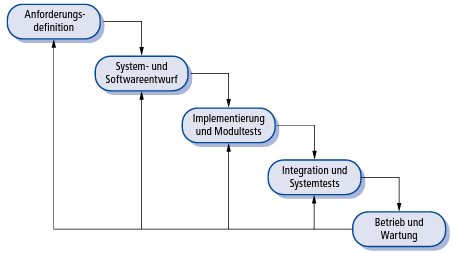
\includegraphics[width=0.5\linewidth]{content/images/wasserfallmodell.png}
        \caption{Wasserfallmodell}
        \label{fig:wasserfallmodell}
      \end{center}
\end{figure}

\subsubsection{Phasen}
Wie in der \fref{fig:wasserfallmodell} zu sehen ist, besteht das Modell grundsätzlich aus den folgenden 5 Phasen.
  \begin{itemize}
      \item Analyse und Definition:\\
      Die Dienstleistungen, Einschränkungen und Ziele des Systems werden in Zusammenarbeit mit den Systembenutzern aufgestellt. Dann werden sie detaillierter  definiert und dienen so als Systemspezifikationen. 
      \item System- und Softwareentwurf:\\  Der Systementwurfsprozess weist die Anforderungen entweder Hard- oder Softwaresystemen zu. So wird eine übergeordnete Systemarchitektur festgelegt. Beim Softwareentwurf geht es um das Erkennen und Beschreiben der grundlegenden abstrakten Softwaresysteme und ihrer Beziehungen zueinander. 
      \item Implementierung und Modultests:\\  In dieser Phase wird der Softwareentwurf durch eine Menge von Programmen oder Programmeinheiten umgesetzt. Das Testen der Module stellt sicher, dass je de Einheit ihre Spezifikation erfüllt.
      \item Integration und Systemtest:\\  Die einzelnen Programmeinheiten oder Programme werden integriert und als Ganzes getestet, um sicherzustellen, dass die Softwareanforderungen erfüllt werden. Nach den Tests wird das Softwaresystem an den Kunden ausgeliefert.
      \item Betrieb und Wartung:\\ Normalerweise ist dies die längste Phase innerhalb des Lebenszyklus. Das System wird installiert und zum Gebrauch freigegeben. Zur Wartung gehören das Korrigieren von Fehlern,  die in den früheren Phasen nicht entdeckt wurden, die Verbesserung der Implementierung von Systemeinheiten und die Verbesserung des Systems, falls neue Anforderungen aufgedeckt werden
  \end{itemize}

Für die Semesterarbeit sind vor allem die Phasen 1-4 von zentraler Bedeutung.

\subsubsection{Planung der Phasen}
Die Detailplanung wird im DevOps mittels des dort verfügbaren Planungssystem, dem ''Delivery Plans'', erstellt und verwaltet. So können die noch zu erledigenden Arbeiten als Issue erfasst werden und sind dann in der entsprechenden Phase sichtbar.\\
Die vier Phasen werden hier in der Monatsansicht abgebildet. Die Milestones sind entsprechenden den bekannten Daten markiert.

\vspace*{3mm}

\begin{figure}[H]
    \begin{center}
        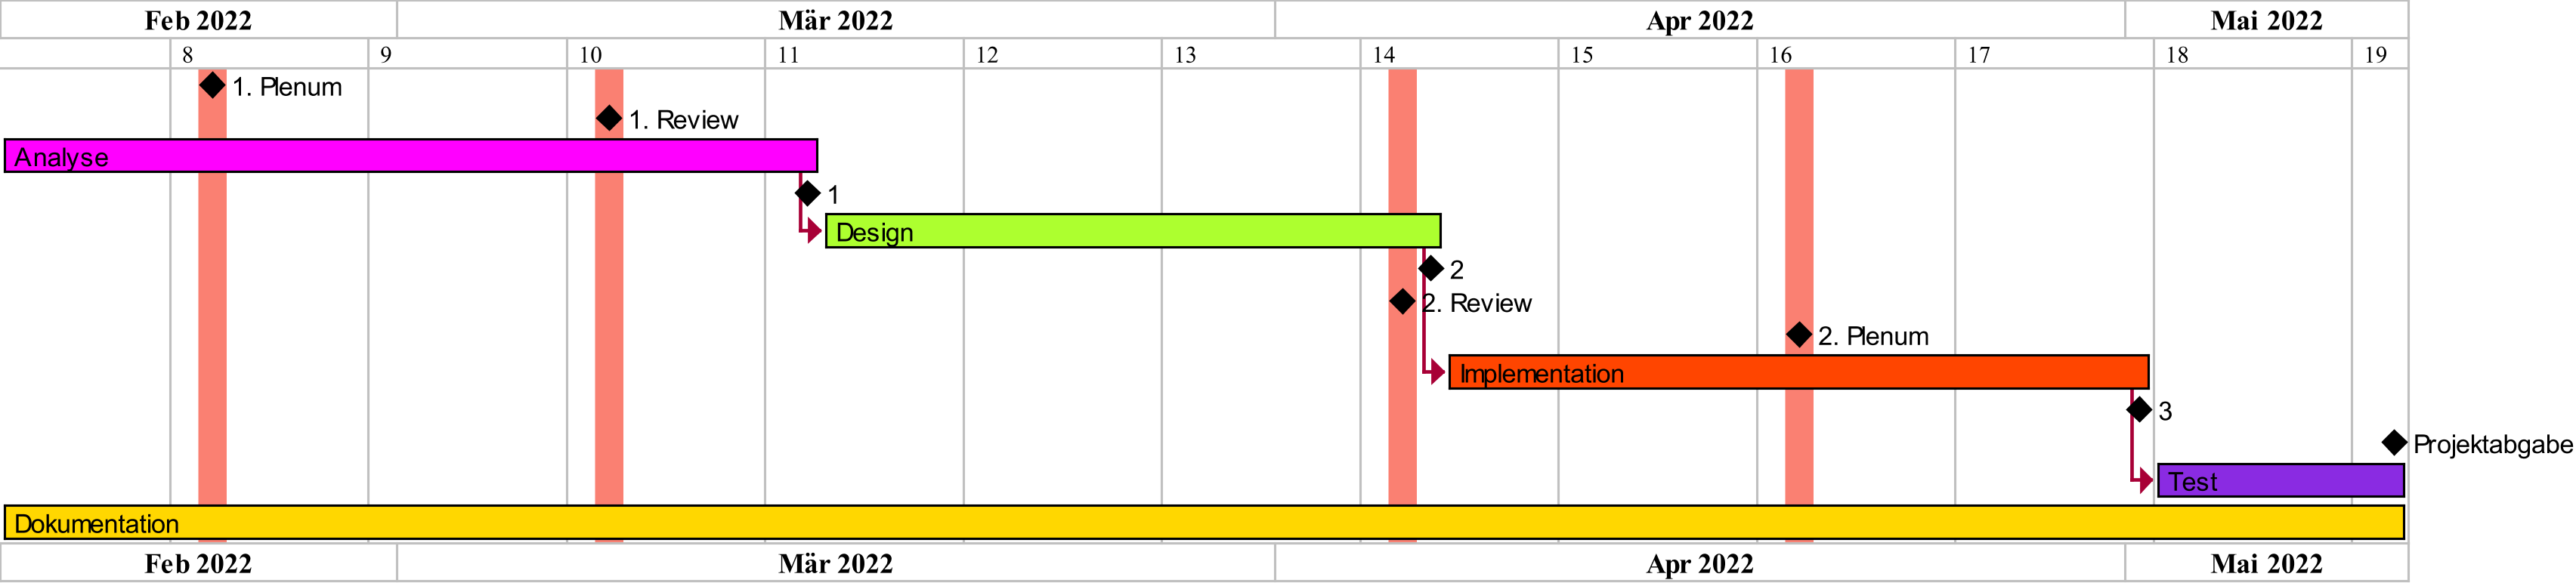
\includegraphics[width=0.95\linewidth]{content/diagrams/out/planning/planning.png}
        \caption{GANT-Diagramm Planung}
      \end{center}
\end{figure}
\newpage

\subsection{Qualitätsmanagement}
Zum sicherstellen der Qualität werden 2 Reviews mit dem Auftraggeber ausgeführt, in welchen der aktuelle Stand des Projektes besprochen wird und eventuelle Massnahmen ergriffen werden können. \\
Zur Qualitätssicherung der Anforderungen der Applikation werden entsprechende Testfälle erstellt und die Applikation damit verifiziert. Wo Programmiertechnisch machbar, sollen automatisierte Tests erstellt und ausgeführt werden. Um die Nichtfunktionalen Anforderungen zu testen, werden Benutzertests durchgeführt. Dabei werden die zukünftigen Benutzer der Applikation miteinbezogen. Informationen zu den definierten Testfällen siehe Kapitel \ref{testkonzept}.

\newpage
\section{Analyse}
\subsection{Risikoanalyse}
Das Risiko berechnet sich durch Multiplikation der Eintrittswahrscheinlichkeit und der Auswirkung. \\

\begin{table}[H]
  \centering
  \settowidth\tymin{\textbf{Auswirkung}}
  \setlength\extrarowheight{2pt}
  \begin{tabulary}{1.0\textwidth}{LCL}
    \textbf{Auswirkung} & &
    \textbf{Eintrittswahrscheinlichkeit} \\
    1 = Unbedeutend\newline 2 = Gering \newline 3 = Moderat \newline 4 = Bedeutend \newline 5 = Katastrophal && 1 = Sehr unwahrscheinlich\newline  2 = Unwahrscheinlich\newline 3 = Möglich\newline 4 = Wahrscheinlich\newline 5 = Sehr Wahrscheinlich\\
  \end{tabulary}
\end{table}

\begin{table}[H]
  \centering
  \settowidth\tymin{\textbf{Auswirkung}}
  \setlength\extrarowheight{2pt}
  \begin{tabulary}{1.0\textwidth}{|C|L|L|C|C|C|}
    \hline
    \rowcolor[HTML]{fdebd0}
    \textbf{Nr.} & 
    \textbf{Risikobeschreibung} & 
    \textbf{Kategorie}& 
    \textbf{Eintrittswahr-scheinlichkeit} & 
    \textbf{Auswirkung} & 
    \textbf{Risiko}\\
    \hline
    1 & Der Zeitplan kann nicht eingehalten werden & Organisatorisch & 3 & 4 & \cellcolor[HTML]{FF0000} 12\\
    \hline
    2 & Das Knowhow zum umsetzen des Projektes ist nicht vorhanden & Personell & 2 & 4 & \cellcolor[HTML]{FFC000}8\\
    \hline
    3 & Durch Krankheit bedingter Personalausfall  & Personell & 2  & 4 & \cellcolor[HTML]{FFC000}8\\
    \hline
    4 & Die neue Software wird vom Endnutzer nicht akzeptiert & Projektmanagement & 2 & 5 & \cellcolor[HTML]{FF0000}10\\
    \hline
    5 & Es werden falsche Anforderungen umgesetzt & Projektmanagement & 2 & 3 & \cellcolor[HTML]{92D050}6\\
    \hline
    6 & Das abspeichern / hinzufügen von Daten dauert zu lange & Technisch & 2 & 2 & \cellcolor[HTML]{00B050}4\\
    \hline
    7 & Verwendete NuGet-Pakete weisen Fehler auf oder werden nicht mehr unterstützt & Technisch & 2 & 3 & \cellcolor[HTML]{92D050}6\\
    \hline
    8 & Die Anforderungen an die Applikation ändern sich & Organisatorisch & 1 & 4 & \cellcolor[HTML]{00B050}4\\
    \hline
  \end{tabulary}
  \caption{Risikoanalyse}
  \label{Risikoanalyse}
\end{table}

\begin{table}[H]
  \centering
  \settowidth\tymin{\textbf{Massnahme}}
  \setlength\extrarowheight{2pt}
  \begin{tabulary}{1.0\textwidth}{|C|L|L|}
    \hline
    \rowcolor[HTML]{fdebd0}
    \textbf{Nr.} & 
    \textbf{Risikobeschreibung} & \textbf{Massnahme}\\
    \hline
    1 & Der Zeitplan kann nicht eingehalten werden & Zeitplanung täglich aktualisieren. So kann der fortschritt des Projektes überprüft werden. Sobald Abweichungen festgestellt werden, muss die Planung angepasst und weitere Massnahmen ergriffen werden\\
    \hline
    2 & Das Knowhow zum umsetzen des Projektes ist nicht vorhanden & Für den Prototypen wird eine schon bekannte Technologie eingesetzt\\
    \hline
    3 & Durch Krankheit bedingter Personalausfall & Genügend Puffer einplanen, Stakeholder zeitlich Informieren\\
    \hline
    4 & Die neue Software wird vom Endnutzer nicht akzeptiert & Die Endbenutzer werden von Anfang an miteinbezogen und sobald erste Prototypen vorhanden sind, wird dies mit den Usern besprochen.\\
    \hline
    5 & Es werden falsche Anforderungen umgesetzt & Pflichtenheft genau Ausarbeiten \\
    \hline
    6 & Das abspeichern / hinzufügen von Daten dauert zu lange & Richtige Konfiguration der Datenbank sicherstellen\\
    \hline
    7 & Verwendete NuGet-Pakete weisen Fehler auf oder werden nicht mehr unterstützt & Nur NuGet-Pakete verwenden die aktuell und weit verbreitet sind\\
    \hline
    8 & Die Anforderungen an die Applikation ändern sich & ImmoGlobal über mögliche Konsequenzen von Nachträglichen Änderungen an den Anforderungen Informieren \\
    \hline
  \end{tabulary}
  \caption{Massnahmen}
  \label{Massnahmen}
\end{table}

\subsection{Stakeholderanalyse}
Die verschiedenen Stakeholder an diesem Projekt haben verschiedene Interessen, die es während dem gesamten Projekt zu berücksichtigen gilt. Als Stakeholder sind all jene gemeint, welche direkt oder indirekt mit dem System in Kontakt stehen. Besonderes Augenmerk sollte auf die Stakeholder welche direkt mit dem System in Verbindung kommen werden, gelegt werden.
Um die verschiedenen Stakeholder aufzuzeigen, werden diese in 2 verschiedene Gruppen eingeteilt.

\subsubsection{Stakeholder mit direkten Interessen}
Diese Gruppe beinhaltet die Stakeholder, welche direkt mit der Applikation arbeiten werden.

\begin{itemize}
  \item Auftraggeber
  \item Mitarbeiter:innen
  \item Hauswartungspersonen
  \item Investoren/Eigentümer der Mietobjekte
\end{itemize}

\subsubsection{Stakeholder mit indirekten Interessen}

\begin{itemize}
  \item Gesetzgeber und Behörden
  \item Mietparteien
  \item Lieferanten
\end{itemize}
\newpage
\subsection{Stakeholderbewertung}
Damit der Einfluss der einzelnen Stakeholder besser bewertet werden kann, wir deren Macht und Einfluss und das Interesse in einer Tabelle festgehalten.

\begin{table}[H]
  \newcolumntype{a}{>{\columncolor[HTML]{fdebd0}}L}
  \newcolumntype{z}{>{\columncolor[HTML]{e8daef}}L}
  \centering
  \settowidth\tymin{\textbf{Stakeholder}}
  \setlength\extrarowheight{2pt}
  \begin{tabulary}{1.0\textwidth}{|L|L|L|a|z|}
    \hline
    \cellcolor[HTML]{e6f2ff}\textbf{Stakeholder} & 
    \cellcolor[HTML]{e6f2ff}\textbf{Beschreibung} & 
    \cellcolor[HTML]{fadbd8}\textbf{Erwartung}& 
    \textbf{Macht und Einfluss} & 
    \textbf{Interesse}\\
    \hline
    Auftraggeber & 
    Geschäftsführung von ImmoGlobal& 
    Einfache, dem Bedürfnis von ImmoGlobal entsprechende Software, welche auf das Wachstum der Firma angepasst ist. &
    7 &
    5 \\ 
    \hline
    Mitarbeiter:innen & 
    Mitarbeiter:innen von ImmoGlobal an den 3 Standorten & 
    Einfache, leicht zu bedienende Software&
    8 &
    8 \\
    \hline
    Hauswartungs-personen & 
    Hauswarte im Dienst von ImmoGlobal &
    Einfaches auffinden der Objekte durch eindeutige Kennzeichnung &
    5 &
    6 \\
    \hline
    Investoren/ Eigentümer der Mietobjekte & 
    Personen/ Juristische Personen welchen die Immobilie gehört &
    Keine Besonderen Erwartungen, Kosten dürfen nicht erhöht werden &
    1 &
    1 \\
    \hline
    Gesetzgeber und Behörden &
    Mietgesetz, Steuerbehörde &
    Gesetze werden eingehalten &
    5 &
    1 \\
    \hline
    Mietparteien & 
    Mieter der Objekte von ImmoGlobal &
    Korrekte Übergabeprotokolle &
    1 &
    2 \\
    \hline
    Lieferanten & 
    Firmen, welche Aufträge von ImmoGlobal ausführen &
    Schnelle Abwicklung der Zahlungen &
    1 &
    2 \\
    \hline
  \end{tabulary}
  \caption{Stakeholderbewertung}
  \label{Stakeholderbewertung}
\end{table}

\begin{figure}[H]
  \begin{center}
      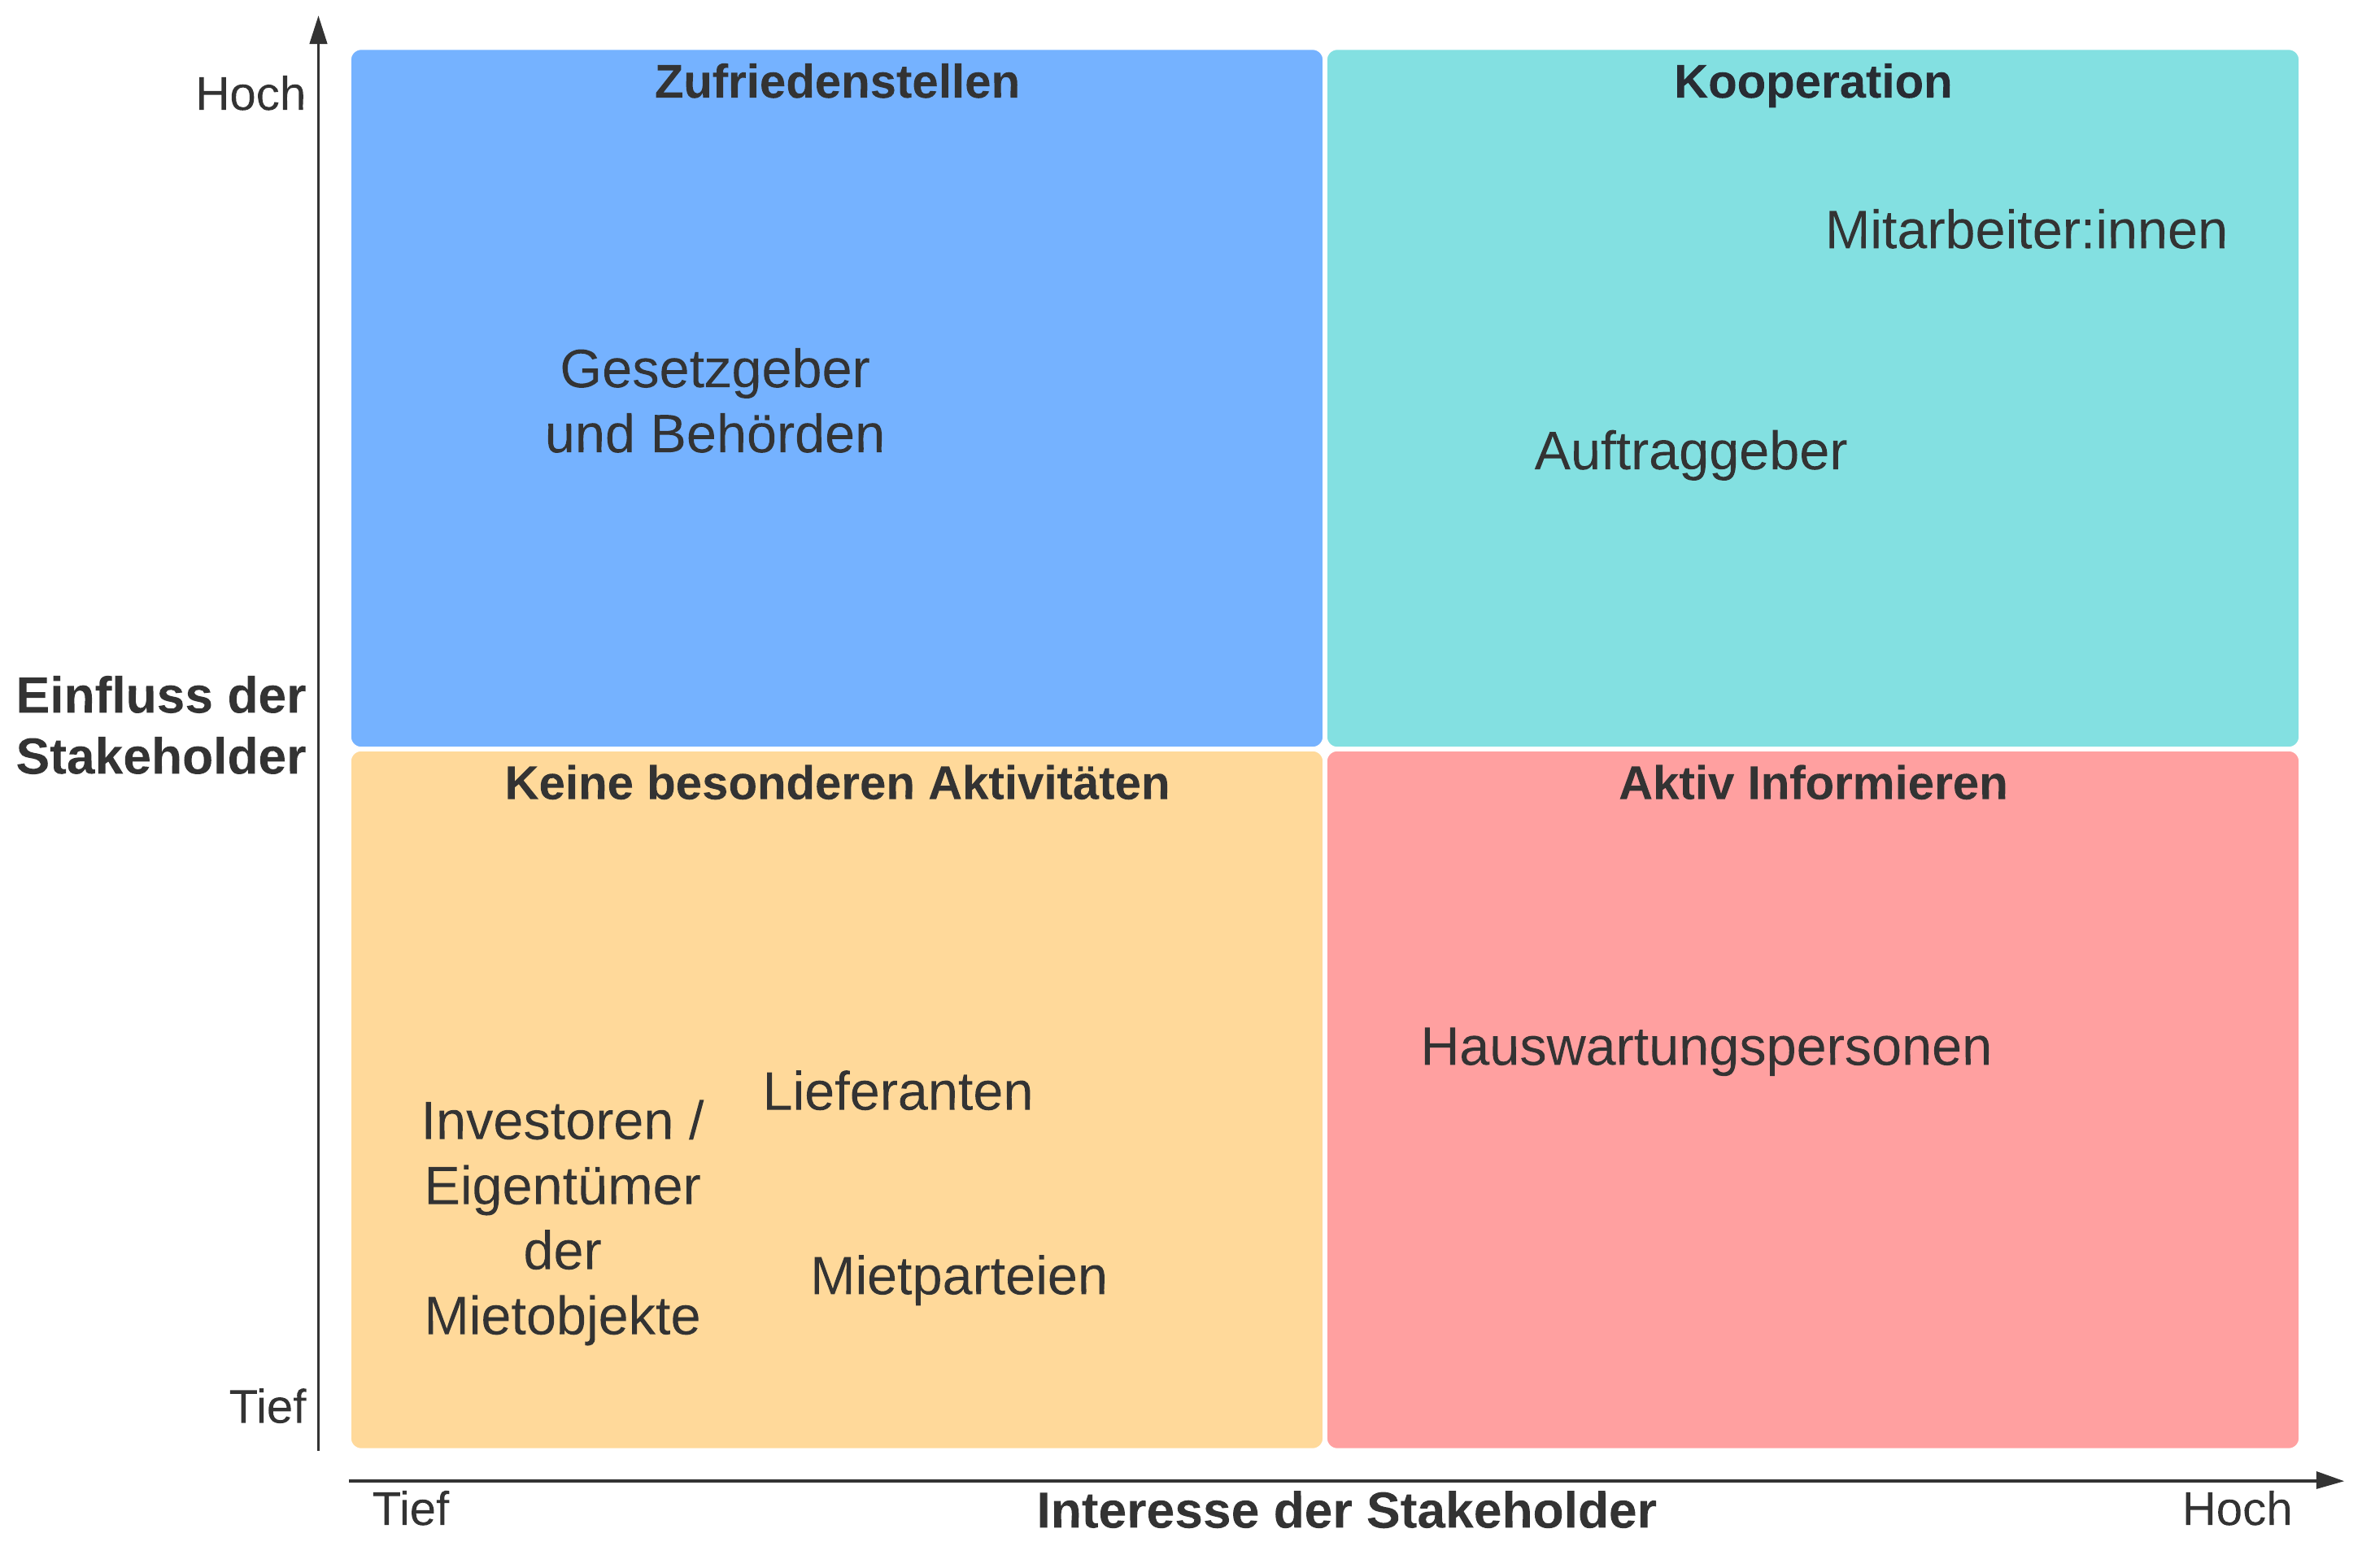
\includegraphics[width=0.58\textwidth]{content/images/Stakeholdematrix.png}
      \caption{Stakeholdermatrix}
      \label{fig:Stakeholdermatrix}
    \end{center}
\end{figure}

Wie aus der Stakeholderanalyse hervorgeht, ist besonders auf die Nutzer der Software zu achten. Das Risiko ist bei den Nutzern vor allem die Akzeptanz der Software. Um dieses Risiko möglichst gering zu halten, müssen die zukünftigen Nutzer von Anfang an in den Entwicklungsprozess mittels WireFrames und ersten Prototypen mit eingebunden werden.

\subsection{Anforderungsanalyse}
\subsubsection{Funktionale Anforderungen}
\begin{table}[H]
  \centering
  \settowidth\tymin{\textbf{Prio}}
  \setlength\extrarowheight{2pt}
  \begin{tabulary}{1.0\textwidth}{|m{16cm}|L|}
    \hline
    \textbf{Datenhaltung}&\textbf{Prio}\\
    \hline
      Die Daten der Applikation müssen in einer Datenbank gespeichert werden & 1\\
    \hline
  \end{tabulary}
  \caption{FA-Datenhaltung}
  \label{faDatenhaltung}
\end{table}

\begin{table}[H]
  \centering
  \settowidth\tymin{\textbf{Prio}}
  \setlength\extrarowheight{2pt}
  \begin{tabulary}{1.0\textwidth}{|m{16cm}|L|}
    \hline
    \textbf{Mietverträge verwalten}&\textbf{Prio}\\
    \hline
    In der Applikation müssen die Mietverträge mit folgenden Angaben erstellt werden können:
    \begin{itemize}
      \item Welcher Mieter:in, bei Wohngemeinschaften/Ehepaaren muss es möglich sein mehrere Mieter pro Mietvertrag zu erfassen
      \item Welche Liegenschaft / Objekt
      \item Der Mietbeginn und gegebenenfalls Mietende
      \item Der Monatlicher Mietzins und die monatlichen Nebenkosten
      \item Die Art der Nebenkosten (Pauschal bzw. à-Konto)
      \item Eine Auflistung der Kostenarten, welche über die Nebenkosten abgerechnet werden (Heiz-, Warmwasseraufbereitungs-, Wasser-, Hauswart-, Treppenreinigungs-, Gartenarbeits-, Strom-, Lift-, Kabelfernsehkosten sowie Abwasser- Kehrichtgebühren)
      \item Ob ein Mietdepot eingerichtet wurde und wenn ja der Depotbetrag in CHF
    \end{itemize}  & 1\\ 
    \hline
  \end{tabulary}
  \caption{FA-Mietverträge}
  \label{faMietverträge}
\end{table}

\begin{table}[H]
  \centering
  \settowidth\tymin{\textbf{Prio}}
  \setlength\extrarowheight{2pt}
  \begin{tabulary}{1.0\textwidth}{|m{16cm}|L|}
    \hline
    \textbf{Liegenschaft erfassen}&\textbf{Prio}\\
    \hline
    Die Liegenschaft muss mit folgenden Informationen in der Applikation erfasst werden können:
    \begin{itemize}
      \item Eine Identifikationsnummer der Liegenschaft
      \item Eine Bezeichnung der Liegenschaft
      \item Die Liegenschaftsadresse
      \item Wie viele Objekte pro Kategorie in der Liegenschaft vorhanden sind. Objektkategorie pro Liegenschaft sind: Wohnung, Raum, Garage, Parkplatz
      \item Abgeschlossene Versicherungen für die Liegenschaft
      \item Die zuständige Hauswartungsperson
    \end{itemize} & 1\\ 
    \hline
  \end{tabulary}
  \caption{FA-Liegenschaft erfassen}
  \label{faLiegenschaftErfassen}
\end{table}

\begin{table}[H]
  \centering
  \settowidth\tymin{\textbf{Prio}}
  \setlength\extrarowheight{2pt}
  \begin{tabulary}{1.0\textwidth}{|m{16cm}|L|}
    \hline
    \textbf{Objekt erfassen}&\textbf{Prio}\\
    \hline
    Ein Objekt muss mit folgenden Informationen in der Applikation erfasst werden können:
    \begin{itemize}
      \item Eine Identifikationsnummer des Objekts
      \item Eine Bezeichnung des Objekts
      \item Die Lage des Objekts. Z.B. 1. OG links
      \item Die Anzahl der Zimmer beim Objekttyp Wohnungen
      \item Die Fläche des Objekts
      \item Eine Beschreibung als Freitextfeld
      \item Was für Geräte in dem Objekt vorhanden sind. Z.B. Kühlschrank, Geschirrwaschmaschine, etc.
      \item Die Anzahl aller Schlüssel nach Typ, die zu diesem Objekt vorhanden sind 
    \end{itemize} & 1\\ 
    \hline
  \end{tabulary}
  \caption{FA-Objekt erfassen}
  \label{faObjektErfassen}
\end{table}

\begin{table}[H]
  \centering
  \settowidth\tymin{\textbf{Prio}}
  \setlength\extrarowheight{2pt}
  \begin{tabulary}{1.0\textwidth}{|m{16cm}|L|}
    \hline
    \textbf{Mieter:in erfassen}&\textbf{Prio}\\
    \hline
    Die Mieter müssen mit folgenden Informationen in der Applikation erfasst werden können:
    \begin{itemize}
      \item Der Name und Vorname
      \item Das Geburtsdatum
      \item Der Heimatort
      \item Der Zivilstand
      \item Die vorherige Wohnadresse
      \item Eine Telefonnummer
      \item Eine E-Mail-Adresse
      \item Eine Bankverbindung
    \end{itemize} & 1\\
    \hline
  \end{tabulary}
  \caption{FA-Mieter:in erfassen}
  \label{faMieterinerfassen}
\end{table}

\begin{table}[H]
  \centering
  \settowidth\tymin{\textbf{Prio}}
  \setlength\extrarowheight{2pt}
  \begin{tabulary}{1.0\textwidth}{|m{16cm}|L|}
    \hline
    \textbf{Buchhaltung}&\textbf{Prio}\\
    \hline
      Es muss eine einfache Buchhaltung mit Ein- und Ausgaben geführt werden, wo die Einzahlungen der Mieter:innen (Mietzinse) und die Ausgaben für den Unterhalt und die Reparaturen verbucht werden können.& 1\\
    \hline
  \end{tabulary}
  \caption{FA-Buchhaltung}
  \label{faBuchhaltung}
\end{table}

\begin{table}[H]
  \centering
  \settowidth\tymin{\textbf{Prio}}
  \setlength\extrarowheight{2pt}
  \begin{tabulary}{1.0\textwidth}{|m{16cm}|L|}
    \hline
    \textbf{Kreditoren verwalten}&\textbf{Prio}\\
    \hline
    Es müssen Kreditoren mit folgenden Informationen verwaltet werden können:
    \begin{itemize}
      \item Aktiv oder gesperrt
      \item Eine Adresse
      \item Der Name und Vorname
      \item Die Mehrwertsteuernummer
      \item Eine Telefonnummer und falls vorhanden eine Faxnummer
      \item Eine E-Mail-Adresse
      \item Eine Kontaktperson mit Namen, Vorname, Telefonnummer, E-Mail-Adresse
    \end{itemize} & 1\\
    \hline
  \end{tabulary}
  \caption{FA-Kreditoren verwalten}
  \label{faKreditorenVerwalten}
\end{table}

\begin{table}[H]
  \centering
  \settowidth\tymin{\textbf{Prio}}
  \setlength\extrarowheight{2pt}
  \begin{tabulary}{1.0\textwidth}{|m{16cm}|L|}
    \hline
    \textbf{Rechnungen erstellen}&\textbf{Prio}\\
    \hline
    Es muss eine Rechnung mit folgenden Informationen erstellt werden können: (für den Prototyp ist keine Ausgabe als PDF oder sonstige Datei notwendig.)
    \begin{itemize}
      \item Das Konto
      \item Der Kreditor
      \item Das Rechnungsdatum
      \item Das Fälligkeitsdatum der Rechnung
      \item Der Rechnungszweck
      \item Die betreffende Liegenschaft oder das betreffende Objekt
      \item Der Rechnungsbetrag mit evtl. Rabatt/Skonto, der Betrag Netto
      \item Die Kategorie als Auswahl Nebenkosten oder Allgemein
    \end{itemize} & 1\\
    \hline
  \end{tabulary}
  \caption{FA-Kreditoren verwalten}
  \label{faRechnungenErstellen}
\end{table}

\begin{table}[H]
  \centering
  \settowidth\tymin{\textbf{Prio}}
  \setlength\extrarowheight{2pt}
  \begin{tabulary}{1.0\textwidth}{|m{16cm}|L|}
    \hline
    \textbf{Mietzinskontrolle}&\textbf{Prio}\\
    \hline
    Es muss überprüft werden können, ob die Miete für ein bestimmtes Objekt schon bezahlt wurde und wenn nicht, muss eine Mahnung für den Mieter generiert werden können. (Mietzinsinkasso) & 1\\
    \hline
  \end{tabulary}
  \caption{FA-Mietzinskontrolle}
  \label{faMietzinskontrolle}
\end{table}

\begin{table}[H]
  \centering
  \settowidth\tymin{\textbf{Prio}}
  \setlength\extrarowheight{2pt}
  \begin{tabulary}{1.0\textwidth}{|m{16cm}|L|}
    \hline
    \textbf{Daten verändern}&\textbf{Prio}\\
    \hline
    Es müssen die Daten der Mieter:innen, die Daten je Liegenschaft und die Daten je Objekt verändert werden können. & 1\\
    \hline
  \end{tabulary}
  \caption{FA-Daten verändern}
  \label{faDatenVeraendern}
\end{table}

\begin{table}[H]
  \centering
  \settowidth\tymin{\textbf{Prio}}
  \setlength\extrarowheight{2pt}
  \begin{tabulary}{1.0\textwidth}{|m{16cm}|L|}
    \hline
    \textbf{Login in der Applikation}&\textbf{Prio}\\
    \hline
    Jede Mitarbeiter:in muss sich mit seinem Persönlichen Login in der Applikation einloggen können & 1\\
    \hline
  \end{tabulary}
  \caption{FA-Login in der Applikation}
  \label{faLogininderApplikatio}
\end{table}

\subsubsection{Nichtfunktionale Anforderungen}
\begin{table}[H]
  \centering
  \settowidth\tymin{\textbf{Prio}}
  \setlength\extrarowheight{2pt}
  \begin{tabulary}{1.0\textwidth}{|m{16cm}|L|}
    \hline
    \textbf{Überblick Liegenschaft / Objekte}&\textbf{Prio}\\
    \hline
    Nach der Einführung der Applikation erhält der Benutzer der Applikation direkt nach dem Login eine Übersicht über die zu verwaltenden Liegenschaften und Objekte. & 1\\ 
    \hline
  \end{tabulary}
  \caption{NFA-Überblick Liegenschaft}
  \label{NFAueberblick}
\end{table}

\begin{table}[H]
  \centering
  \settowidth\tymin{\textbf{Prio}}
  \setlength\extrarowheight{2pt}
  \begin{tabulary}{1.0\textwidth}{|m{16cm}|L|}
    \hline
    \textbf{Starten der Applikation}&\textbf{Prio}\\
    \hline
    Das Starten der Applikation sollte nicht länger als 10 Sekunden dauern. Ansonsten muss mit einem Ladebildschirm die Wartezeit überbrückt werden & 3\\ 
    \hline
  \end{tabulary}
  \caption{NFA-Starten der Applikation}
  \label{NFAStarten}
\end{table}

\begin{table}[H]
  \centering
  \settowidth\tymin{\textbf{Prio}}
  \setlength\extrarowheight{2pt}
  \begin{tabulary}{1.0\textwidth}{|m{16cm}|L|}
    \hline
    \textbf{Sicherheit}&\textbf{Prio}\\
    \hline
    Die Passwörter für das Login werden nur verschlüsselt auf der Datenbank abgespeichert damit die Vertraulichkeit gewährleistet ist. & 3\\ 
    \hline
  \end{tabulary}
  \caption{NFA-Sicherheit}
  \label{NFASicherheit}
\end{table}

\begin{table}[H]
  \centering
  \settowidth\tymin{\textbf{Prio}}
  \setlength\extrarowheight{2pt}
  \begin{tabulary}{1.0\textwidth}{|m{16cm}|L|}
    \hline
    \textbf{Änderungsverfolgung}&\textbf{Prio}\\
    \hline
     Um die Änderungen nachverfolgen zu können, wird bei jeder Änderung ein Eintrag in einer Audit-Trail-Tabelle auf der Datenbank geschrieben. & 4\\
    \hline
  \end{tabulary}
  \caption{NFA-Änderungsverfolgung}
  \label{NFAAenderungsverfolgung}
\end{table}

\subsection{Lösungsvarianten}
\subsubsection{Analyse mit Morphologischer Kasten}
\begin{figure}[H]
  \begin{center}
    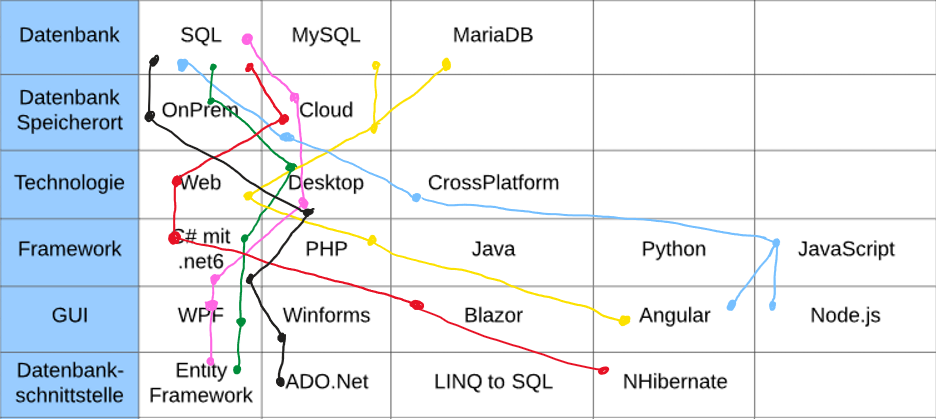
\includegraphics[width=1\linewidth]{content/images/morphoKasten.png}
    \caption{Analyse mit Morphologischem Kasten}
    \label{morphoKasten}
  \end{center}
\end{figure}

Als Lösungsvarianten für die Applikation werden verschiedene Technologien in Betracht gezogen und im Morphologischen Kasten als Parameter hinzugefügt. Wie zu sehen ist, gibt es sehr viele verschiedene Möglichkeiten die verwendet werden könnten. Die dargestellten Lösungspfade sind nicht abschliessend.

\subsubsection{Variantenauswahl}
Als Sinnvolle Lösungsvarianten kommen folgende Möglichkeiten in Frage: 
\begin{itemize}
  \item Webbasierte Applikation mit SQL Datenbank in der Cloud
  \item Applikation mit WPF und .NET, als Datenbankschnittstelle Entity Framework, SQL in der Cloud oder OnPrem
  \item Applikation Windows Forms und .net Framework, als Datenbankschnittstelle Entity Framework, SQL in der Cloud oder OnPrem
\end{itemize}
Ob die Datenbank schlussendlich OnPrem oder in der Cloud verwaltet wird, spielt im Endeffekt für die Applikation keine so Grosse rolle da nur die entsprechende Verknüpfung angepasst werden muss. Wenn die Datenbank aber in der Cloud gehostet wird, muss darauf hingewiesen werden dass zu jeder zeit eine stabile Internetverbindung zum benutzen der Applikation benötigt wird.\\
\vspace*{1mm}

Da die Applikation in Verschiedenen Standorten genutzt werden soll und unter Umständen auch von den Hauswartungspersonen zum Erfassen von Reparaturanträgen oder sonstigen Einträgen verwendet wird, würde sich eine Webbasierte Applikation bestens eignen.\\
Im Rahmen der Semesterarbeit soll aber nur ein Prototyp mit einer schon bekannten Technologie erstellt werden. Aus diesem Grund kommt diese Lösung nicht infrage. Stattdessen wird als Lösung die Variante mit WPF und .NET6 gewählt und als ORM das EntityFramework Core, da in einer früheren Projektarbeit schon erfolgreich ein Projekt mit dieser Technologie umgesetzt wurde.